\setauthor{\firstauthor}
\section{System Architecture and Frontend}\label{sec:implementation:frontend}

\subsection{Overall Architecture}\label{sec:implementation:frontend:architecture}

\begin{figure}[htbp]
	\centering
	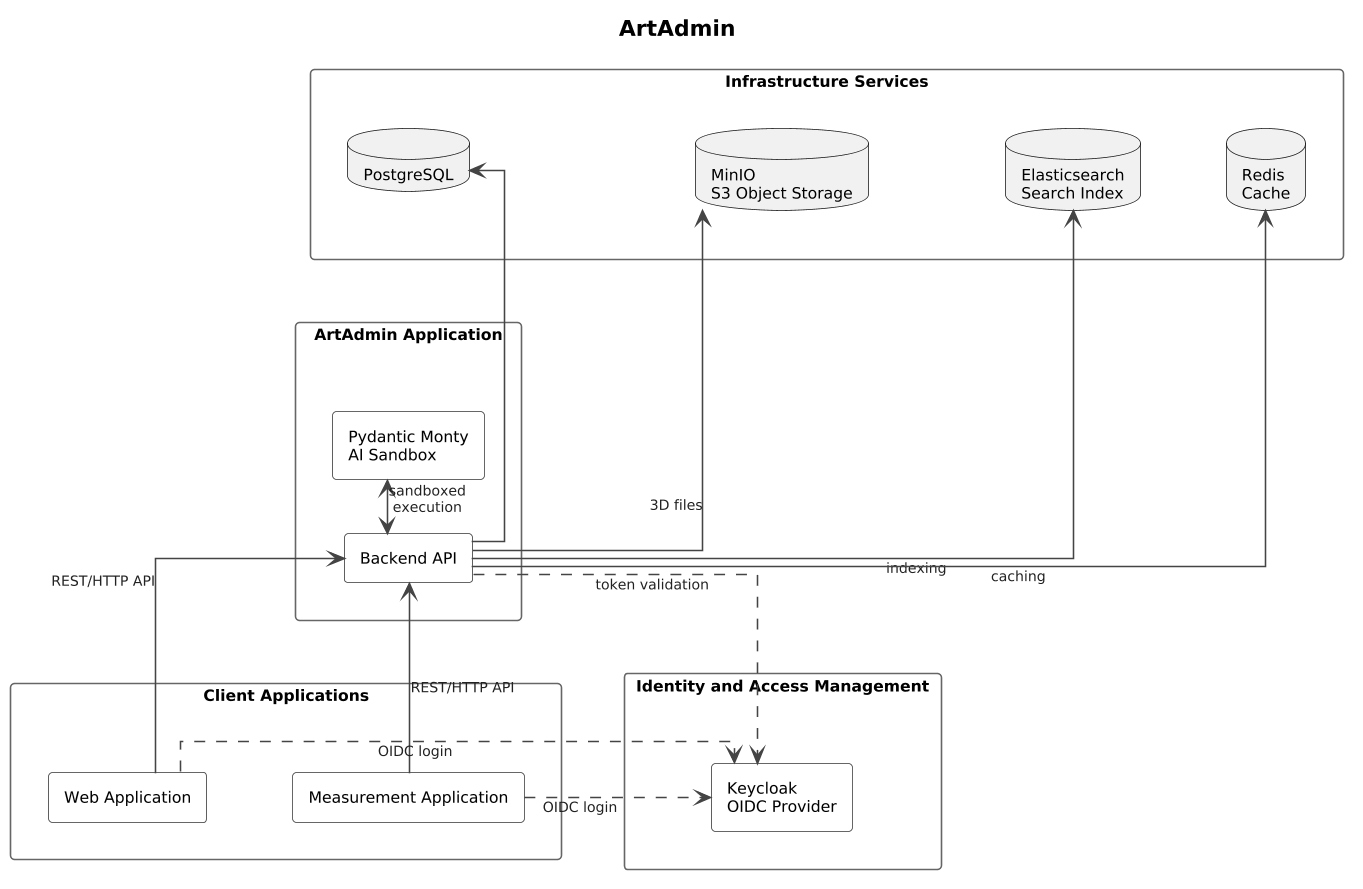
\includegraphics[width=1\textwidth]{pics/component-diagram.png}
	\caption{Component diagram of ArtAdmin. Source: \cite{aiComponentDiagram}}
	\label{fig:component-diagram}
\end{figure}

The component diagram \ref{fig:component-diagram} shows the overall architecture of ArtAdmin. The system is organized into four layers: the client applications layer, the identity and access management layer, the application layer, and the infrastructure service layer. This separation follows the principle of separation of concerns. The client application isolates the presentation layer from the business logic, while the identity and access management layer centralizes the single point of authentication. Furthermore, the infrastructure layer isolates the services that are needed to run this program. This design also allows for horizontal scaling of the backend, because it is stateless, meaning no information is saved directly within the REST application.

The client applications layer consists of a web application, which serves as the main user interface and handles the administration and display of users and information. It also includes ArtMeasure, a desktop application for calculating object measurements based on a 3D camera. Both applications communicate with the backend via a REST API over HTTP, and all user interfaces authenticate through the same OIDC provider, in this case Keycloak.

The application layer, or backend layer, consists of an ASP.NET Core backend, which is the core program handling all traffic and communicating with all services. Furthermore, this layer includes Pydantic Monty, a secure Python interpreter written in Rust for executing code generated by AI agents \cite{pydantic-monty}. This software is used to prevent ArtPilot from executing unauthorized and unsafe code while still enabling the import of any format.

This software solution uses four additional services, all of which can be self-hosted. For storing structured information, we use PostgreSQL. For image and vector data storage, we use MinIO, because it implements the S3 API and can therefore be replaced at any time by another program that also implements this API, such as AWS S3. Furthermore, for the use case of searching information, we use Elasticsearch, because it provides the speed and full-text search capabilities required. Redis is used as a cache for request results to speed up the application; it was chosen because it is a fast, in-memory key-value store, which is a widely used choice for this use case.
\cite{archetecture-cleanup}

\subsection{Frontend Implementation}\label{sec:implementation:frontend:implementation}

\section{Backend and Data Model}\label{sec:implementation:backend}

\subsection{Backend Architecture}\label{sec:implementation:backend:architecture}

\subsection{Object and Provenance Data Model}\label{sec:implementation:backend:data-model}

\subsection{ArtPilot Architecture}\label{sec:implementation:backend:artpilot}

\section{Data Storage and Search}\label{sec:implementation:storage}

\subsection{Database and Media Management}\label{sec:implementation:storage:database}

\subsection{Full-Text Search and Filtering}\label{sec:implementation:storage:search}

\section{Image Similarity Search}\label{sec:implementation:similarity}

\subsection{Processing Pipeline}\label{sec:implementation:similarity:pipeline}

\subsection{Similarity Computation and Robustness}\label{sec:implementation:similarity:robustness}

\section{Depth Camera and 3D Measurement}\label{sec:implementation:camera}

\subsection{Hardware, Software and Measurement Principle}\label{sec:implementation:camera:hardware}

\subsection{Data Quality and Measurement Uncertainty}\label{sec:implementation:camera:quality}

\subsection{Measurement versus Scanning and Limitations}\label{sec:implementation:camera:limitations}

\section{Authentication, Authorization and Auditability}\label{sec:implementation:auth}

\section{Deployment and Operations}\label{sec:implementation:deployment}

\section{Testing Concept and Traceability}\label{sec:implementation:testing}
